
La formación de un trombo en el interior de una arteria se denomina trombosis arterial. Esta formación de coágulos suele desencadenarse con la ruptura de una placa ateroesclerótica. Una placa ateroesclerótica es la manifestación principal de la aterosclerosis, que no es más que la acumulación de grasas, colesterol y otras sustancias dentro de las arterias y en sus paredes. La ruptura de estas placas es un acontecimiento que provoca un entorno favorable a la formación de trombos, al que se incorporan rápidamente las plaquetas.

\begin{figure}[h]
    \centering
	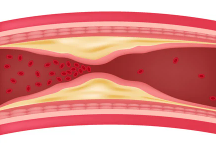
\includegraphics[width=0.70\textwidth]{figures/aterosclerosis.png}
	\caption{Formación de un trombo por aterosclerosis}
	\label{fig:example1}
  \end{figure}
  \textit{La imagen nos la formación de trombos arteriales provocados por aterosclerosis. En amarillo podemos ver las placas ateroscleróticas impidiendo el paso del flujo arterial en rojo}
  
La incorporación de plaquetas al trombo provoca que la cantida de fibrina aumente puesto que actúa como una especie de pegamento o hilo entre las plaquetas. Así, el coágulo aumenta lentamente a medida que el trombo se extiende por la luz arterial. Por ello, un trombo arterial contiene generalmente muchas plaquetas y aumenta rápidamente de tamaño.

Los trombos asociados a la arritmia se forman en entornos de bajo flujo y baja presión, por lo que los coágulos resultantes crecen lentamente y son ricos en fibrina. También se clasifican como trombos arteriales, aunque se asemejan más a los trombos de tipo venoso, cumpliendo así la tríada de Virchow para la trombogénesis:
        \begin{enumerate}
          \item Lesión endotelial.
          \item Lentitud del flujo o estasis sanguínea.
          \item Estados de hipercoagulabilidad.
         \end{enumerate}

Este tipo de coágulo sanguíneo puede causar ataques cardiacos bastante graves, si el taponamiento es en las arterias coronarias, o accidentes cerebrovasculares (en ocasiones irreversibles), si el taponamiento es en arterias cerebrales. La trombosis arterial es muy dañina para el organismo y, en general, mucho más grave y urgente que la trombosis venosa debido a la falta de oxígeno que provoca el taponamiento de las arterias en aquellos lugares donde están ubicadas. 
	
\section{Genes Asociados}
		La trombosis arterial se ve afectada por diversos genes. Este mapa nos muestra las interacciones entre los 25 genes que intervienen.
		
    \begin{figure}[h]
        \centering
    	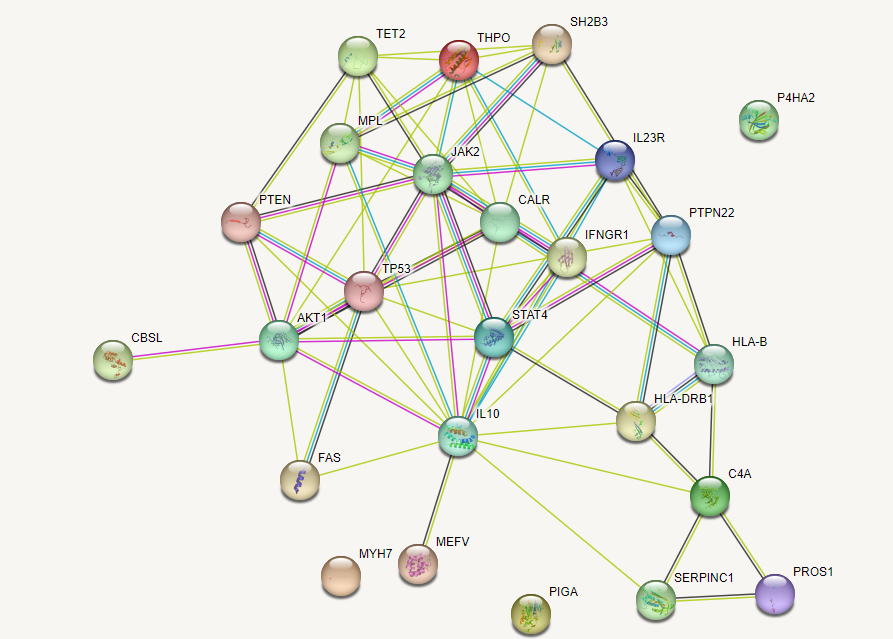
\includegraphics[width=0.70\textwidth]{figures/genes_asociados.png}
    	\caption{Genes asociados en la trombosis}
    	\label{fig: Figura 2}
      \end{figure}
    \textit{La imagen nos representa los genes asociados a la trombosis arterial en círculos con sus respectivos nombres. Además también nos representa las iteracciónes entre ellos en líneas de colores.}
\subsection{\textbf {JAK2, STAT4}}

          El gen JAK2 es relevante, ya que como podemos ver en la Figura \ref{fig: Figura 2}  participa en multitud de interacciones entre genes. Para explicar el funcionamiento de este gen es necesario explicar las quinasas Janus, tipología de la JAK2.\\
		
		Las quinasas Janus están en el origen de diversas respuestas inmunológicas e inflamatorias y engloban 4 enzimas intracelulares de tipo tirosina-quinasa (JAK1, JAK2, JAK3 y TYK2 [tyrosine kinase-2]). En este caso, la que interviene en la trombosis es la JAK2. Estas enzimas están asociadas con la región membranosa intracelular de distintos receptores que convierten las señales extracelulares, mediadas por diversas citocinas u hormonas, en procesos intracelulares. La unión de una citocina al receptor causa su dimerización e induce la activación de las JAK asociadas. Cuando esto ocurre, las JAK fosforilan residuos específicos del dominio citoplasmático del receptor, donde se anclan los transductores de señales (STAT). Entonces se produce la fosforilación de los STAT que una vez activados se dimerizan y traslocan al núcleo, donde participan en la expresión de múltiples proteínas.\\
		
		Estas proteína es esencial para mediar las respuestas a la IL10 en los linfocitos, y regular la diferenciación de las células T helper, además de ser de suma importancia en la regulación del equilibrio entre ambas.  La deficiencia de STAT4 da lugar a una reducción de la aterosclerosis a través de la modulación de la función de las células B y del contenido de leucocitos en la aorta. Esta respuesta inmunológica hacia la anomalía de la arterosclerosis, provoca el aumento de leucocitos favoreciendo el taponamiento de glóbulos rojos. Es por ello, que las trombosis arteriales también son denominadas blancas.\\
		
	    La IL10 es una citocina reguladora del sistema inmunitario que actúa sobre muchas células con propiedades antiinflamatorias, capaz de inhibir la síntesis de citocinas proinflamatorias por los linfocitos T y los macrófagos. 
	    Esta al unirse a su receptor, provoca la fosforilación de STAT3 mediada por JAK1 y STAT2
	
	

\section{\textbf {Enfermedades Asociadas}}

\subsection { \textbf{Trombocitosis familiar}}

La trombocitosis familiar es un tipo de trombocitosis, un aumento mantenido del número de plaquetas, que afecta a la línea de progenitores de plaquetas/megacariocitos y puede producir tendencia a trombosis y hemorragia, pero no causa proliferación maligna.

Esta enfermedad está causada por mutaciones en la línea germinal en el gen THPO o e el gen MPL. Dichos genes también están relacionados con la trombosis arterial, además del gen JAK2.

Para diagnosticar esta enfermedad es obligatorio la realización de pruebas genéticas. 



\subsection{\textbf{Trombocitemia esencial}}

La trombocitemia esencial (TE) es uno de los trastornos mieloproliferativos Ph-negativos más frecuentes. Esta se caracteriza por una elevación mantenida de las plaquetas, debida a la proliferación excesiva de los megacariocitos de la médula ósea.

Las mutaciones somáticas en el gen JAK2 son las alteraciones más comunes, pero también se han encontrado mutaciones en el gen MPL en los casos de TE con mieloproliferación. Menos frecuente, se han identificado mutaciones en el gen CARL en aquellos casos en los que JAK2 y MPL no sufrían mutaciones. 

Esta enfermedad es adquirida pero también se ha observado una forma familiar de trombocitosis familiar.

\subsection{\textbf{Policitemia vera}}

La policitemia vera (PV), es un síndrome mieloproliferativo de carácter adquirido. Está caracterizada por un aumento absoluto de la masa eritrocitaria debido a su proliferación incontrolada que generalmente se asocia a una proliferación, también incontrolada de leucocitos y plaquetas.

La gran mayoría de los pacientes presentan mutaciones en el gen JAK2, causante de proliferación.

\subsection{\textbf{Enfermedad de Behçet}}

La enfermedad de Behcet, es un trastorno poco frecuente que causa la inflamación de los vasos sanguíneos en todo el cuerpo, es decir, una vasculitis multisistémica. Esta es crónica  y recurrente que se caracteriza por lesiones mucocutáneas y manifestaciones arteriales, oculares y del sistema nervioso central.

El antígeno HLA está asociado en el 70\% de los casos.  